% Modelo de slides para projetos de disciplinas do Abel
\documentclass[10pt]{beamer}

\usetheme[progressbar=frametitle]{metropolis}
\usepackage{appendixnumberbeamer}
\usepackage{verbatim}
\usepackage[numbers,sort&compress]{natbib}
\usepackage[ruled,linesnumbered]{algorithm2e}
%\bibliographystyle{plainnat}
%\bibliographystyle{abbrv}
%\bibliographystyle{plain}
\bibliographystyle{ieeetr}

\usepackage{booktabs}
\usepackage{subfigure}
\usepackage[scale=2]{ccicons}
\newcommand{\themename}{\textbf{\textsc{metropolis}}\xspace}
\usepackage{xspace}

\title{Overview of Adversarial Attack}
% \subtitle{Subtítulo}
% \date{\today}
\date{\today}
\author{Pan Meng}
\institute{School of Computer Science, Sun Yat-sen University}
\logo{
\includegraphics[width = 1.5cm]{figure/logo.jpg}}
\titlegraphic{\hfill
\includegraphics[height=1.5cm]{figure/logo.jpg}}

\begin{document}

\maketitle
\begin{frame}[allowframebreaks]{Contents}
  \setbeamertemplate{section in toc}[sections numbered]
  %\tableofcontents[hideallsubsections]
  \tableofcontents
\end{frame}

\section{Attack Methods}
\subsection{white box}

\subsubsection{fgsm}
\begin{frame}
  Explaining and Harnessing Adversarial Examples~\cite{fgsm}\\
  contributions:
  \begin{enumerate}
    \item They demonstrated that the reason why the adversarial examples exist is the linear nature of neural network, rather than the extreme nonlinearity and over fitting of the model proposed in the previous works.
    \item They proposed a fast method to generate adversarial examples named FGSM:
      \begin{align}
        \eta = \epsilon sign(\bigtriangledown_{x}J(\theta, x, y)) .
      \end{align}
  \end{enumerate}
\end{frame}

\subsubsection{I-fgsm}
\begin{frame}
  Adversarial Examples in the Physical World~\cite{ifgsm}\\
  contributions:
  \begin{enumerate}
    \item This paper researched the attack manner in the physical world scene, they  show that adversarial examples exist even in the physical world.
    \item They proposed a basic iterative method that extends FGSM by iteratively taking multiple small gradient steps:
    \begin{align}
      X_0^{adv} = X, X_{N+1}^{adv} = Clip_{X,\epsilon} \{X_{N+1}^{adv} + \alpha sign(\bigtriangledown_{x}J(\theta, x, y))\} . 
    \end{align}
  \end{enumerate}
\end{frame}

\subsubsection{PGD}
\begin{frame}
  Towards Deep Learning Models Resistant to Adversarial~\cite{pgd}\\
  contributions:
  \begin{enumerate}
    \item They address adversarial attack problem through the lens of robust optimization, in particular, they proposed an min-max framework to unify this optimization problem:
    \begin{align}
      min (\mathbb{E}_{(x,y)\sim D} [max \mathcal{L} (\theta, x+\delta, y)] ).
    \end{align}
    \item They proposed a strongest first-order attack method:
    \begin{align}
      x^{t+1} = Proj_{x+s} (x^t + \alpha sign(\bigtriangledown_{x}J(\theta, x, y))).
    \end{align}
    \item They show experimentally that network capacity plays a crucial role in enabling
    robustness.
  \end{enumerate}
\end{frame}

\subsubsection{Robustness and Accuracy}
\begin{frame}
  Is Robustness the Cost of Accuracy? – A Comprehensive Study on the Robustness of 18 Deep Image Classification Models~\cite{raa}\\
  contributions:
  \begin{enumerate}
    \item They present the first comprehensive study that compares the robustness of
    18 popular models, offering a complete picture of the accuracy v.s. robustness trade-off.
    \item They find that robustness is scarified when solely pursuing a higher classification accuracy.
    \item They find that network architecture has a larger impact on robustness than model size.
    \item The adversarial examples generated by the VGG family can transfer very well
    to all the other 17 models, while most adversarial examples of other models can
    only transfer within the same model family.
  \end{enumerate}
\end{frame}

\subsubsection{Deepfool}
\begin{frame}
  DeepFool: A Simple and Accurate Method to Fool Deep Neural Networks~\cite{deepfool}\\
  contributions:
  \begin{enumerate}
    \item They proposed an accurate method to quantify the robustness of classifiers.
    \item They proposed deepfool method to generate adversarial examples, with which the 
    robustness of classifier is significantly increased.
    \item We show that using imprecise approaches for the computation of adversarial 
    perturbations could lead to different and sometimes misleading conclusions about 
    the robustness.
  \end{enumerate}
\end{frame}

\subsubsection{CW}
\begin{frame}
  Towards Evaluating the Robustness of Neural Networks~\cite{cw}\\
  contributions:
  \begin{enumerate}
    \item They introduced three new attacks for the $L_0$, $L_2$, and $L_{\infty}$
    distance metrics, in which $L_0$ attack is the first published attack on ImageNet.
    \begin{align}
      minimize \| \frac{1}{2}(tanh(w)+1) - x \|_{2}^{2} + c\cdot f(\frac{1}{2}(tanh(w)+1)) 
    \end{align}
    \begin{align}
      f(x^{'}) = max(max{Z(x^{'})_i:i \neq t} - Z(x^{'})_t, -k)
    \end{align}
    \item They evaluate the choice of the objective function for finding adversarial examples, and show that
    the choice can dramatically impact the efficacy of an attack.
  \end{enumerate}
\end{frame}
\subsection{MDE Attack}
\begin{frame}
  Targeted Adversarial Perturbations for Monocular Depth Prediction!\cite{nipsmdeattack}\\
  \begin{figure}
  \centering
  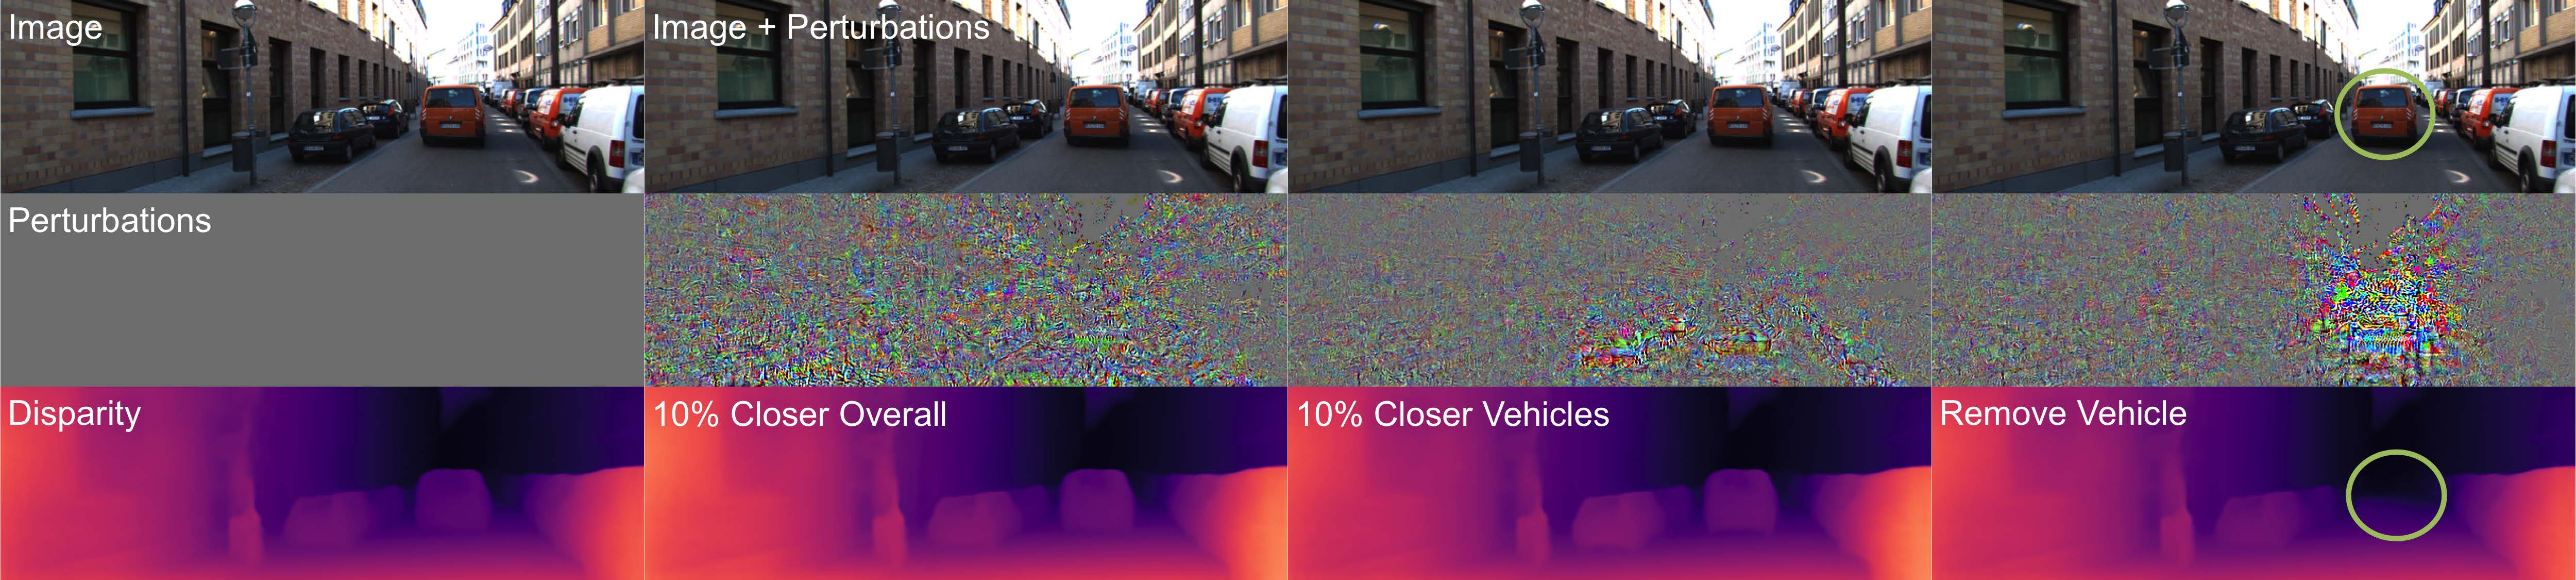
\includegraphics[width=1\linewidth]{figure/Targeted Adversarial Perturbations for Monocular Depth Prediction_NIPS2020.jpg}
  \caption{Altering the predicted scene with adversarial perturbations.}
  \end{figure}
  contributions:
  \begin{enumerate}
    \item They proposed a attack method for MDE, and examine it on
    Monodepth, Monodepth2, PackNet, VNL.
    \item They show perturbations for altering entire predictions to a target
    scene.
    \item They show localized attacks on specific categories and object instances.
    \item They discuss the transferabilty of such perturbations.
  \end{enumerate}
\end{frame}

\begin{frame}
  attack method:
  \begin{algorithm}[H]
    \caption{Proposed attack method for a regression task.}
    \label{alg:attack mde}
    Parameters: learning rate$\eta $,noise upper norm $\xi $\;
    \KwIn{Image $x$, target depth map $d_{(x)}$, depth network $f_d$.}\
    Initialization: $v_0(x)$\\
    \For(){n$\le$ N}{
      $v_{n+1}(x)=\lceil v_n(x) - \eta \nabla \mathcal{L}(x, v_n(x), d_{(x)}, f_d)\rceil $
    }
    \KwOut{Perturbation $v_N(x)$}
\end{algorithm}
 $\mathcal{L}(x, v_n(x), d_{(x)}, f_d) = \frac{\left\lVert f_d(x+v(x))-d(x)\right\rVert_1 }{d(x)}$ 
\end{frame}
\subsection{black box}
  
\section{Defense Methods}

\section{Summary}
\subsection{20210917}
\begin{frame}
  FastDepth: Fast Monocular Depth Estimation on Embedded Systems~\cite{fastdepth}
  \begin{figure}
    \centering
    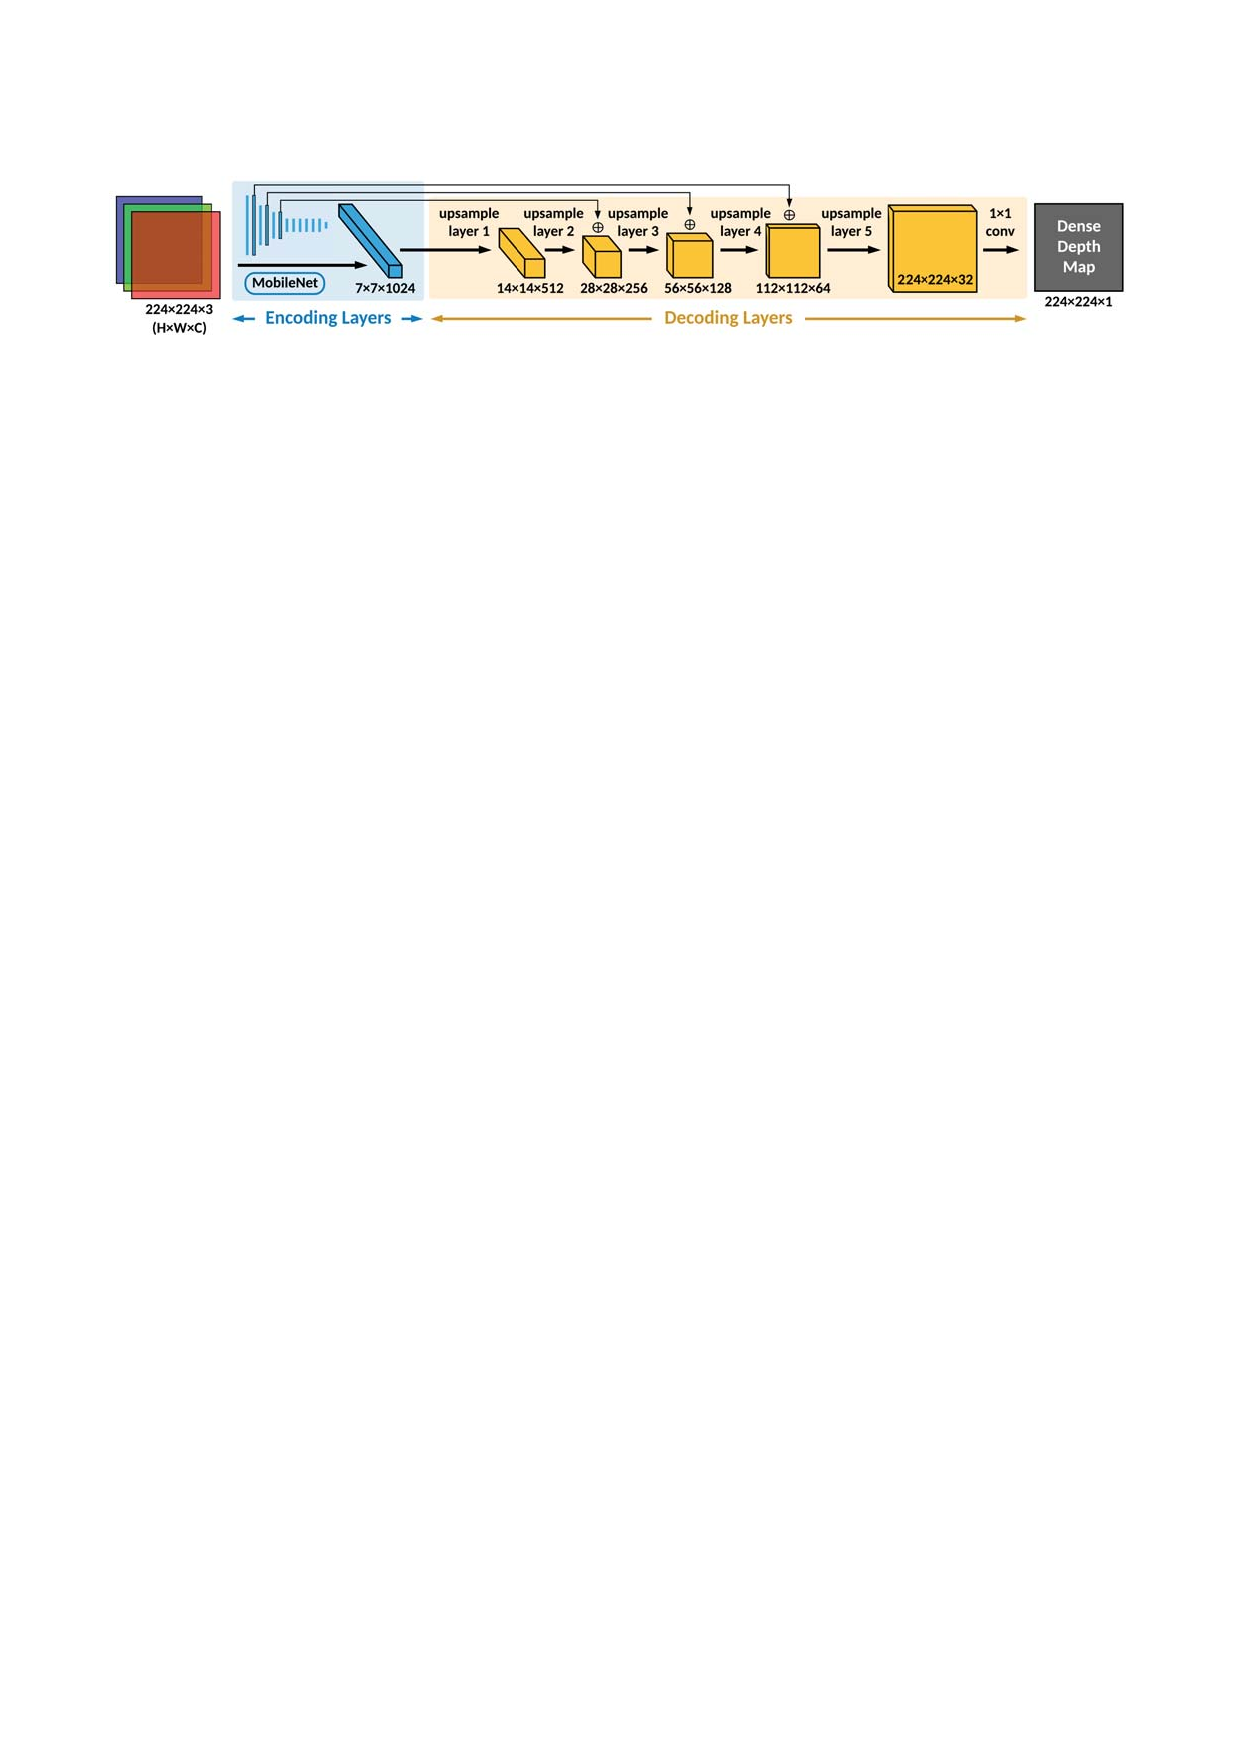
\includegraphics[width=1\linewidth]{figure/20210917/FastDepth_Architecture.pdf}
    \caption{Architecture of fastdepth}
  \end{figure}
\end{frame}
\begin{frame}
  I obtained some results produced by their pretrained model, which will be
  used as attack target later.
  \begin{figure}
      \subfigure[]{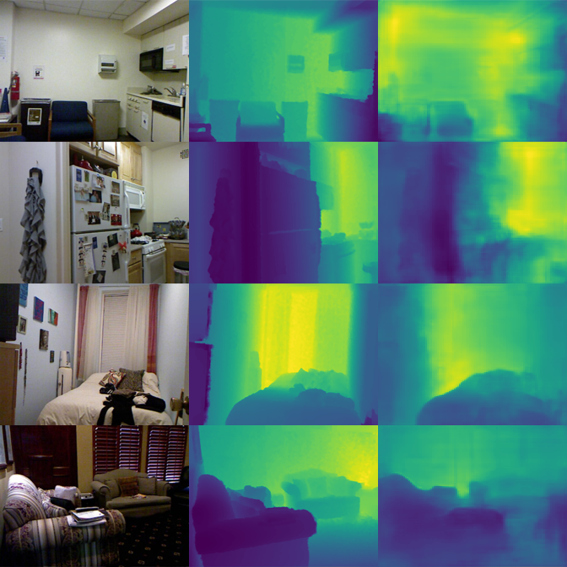
\includegraphics[width=0.45\linewidth]{figure/20210917/fastdepth_result1.png}}
      \subfigure[]{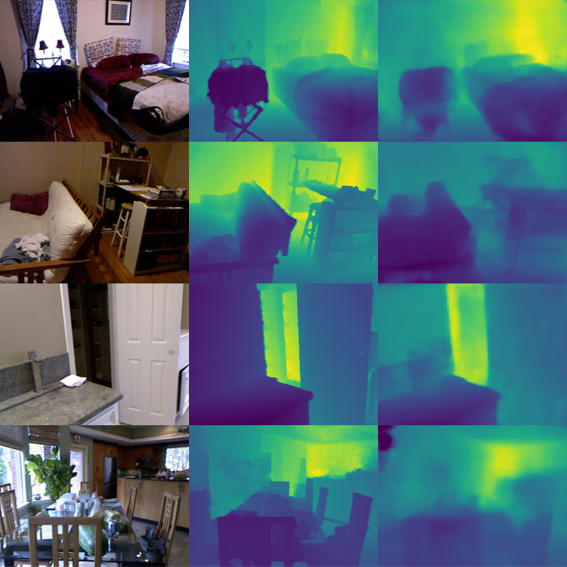
\includegraphics[width=0.45\linewidth]{figure/20210917/fastdepth_result2.png}}
  \end{figure}
\end{frame}
\begin{frame}
  \begin{figure}
    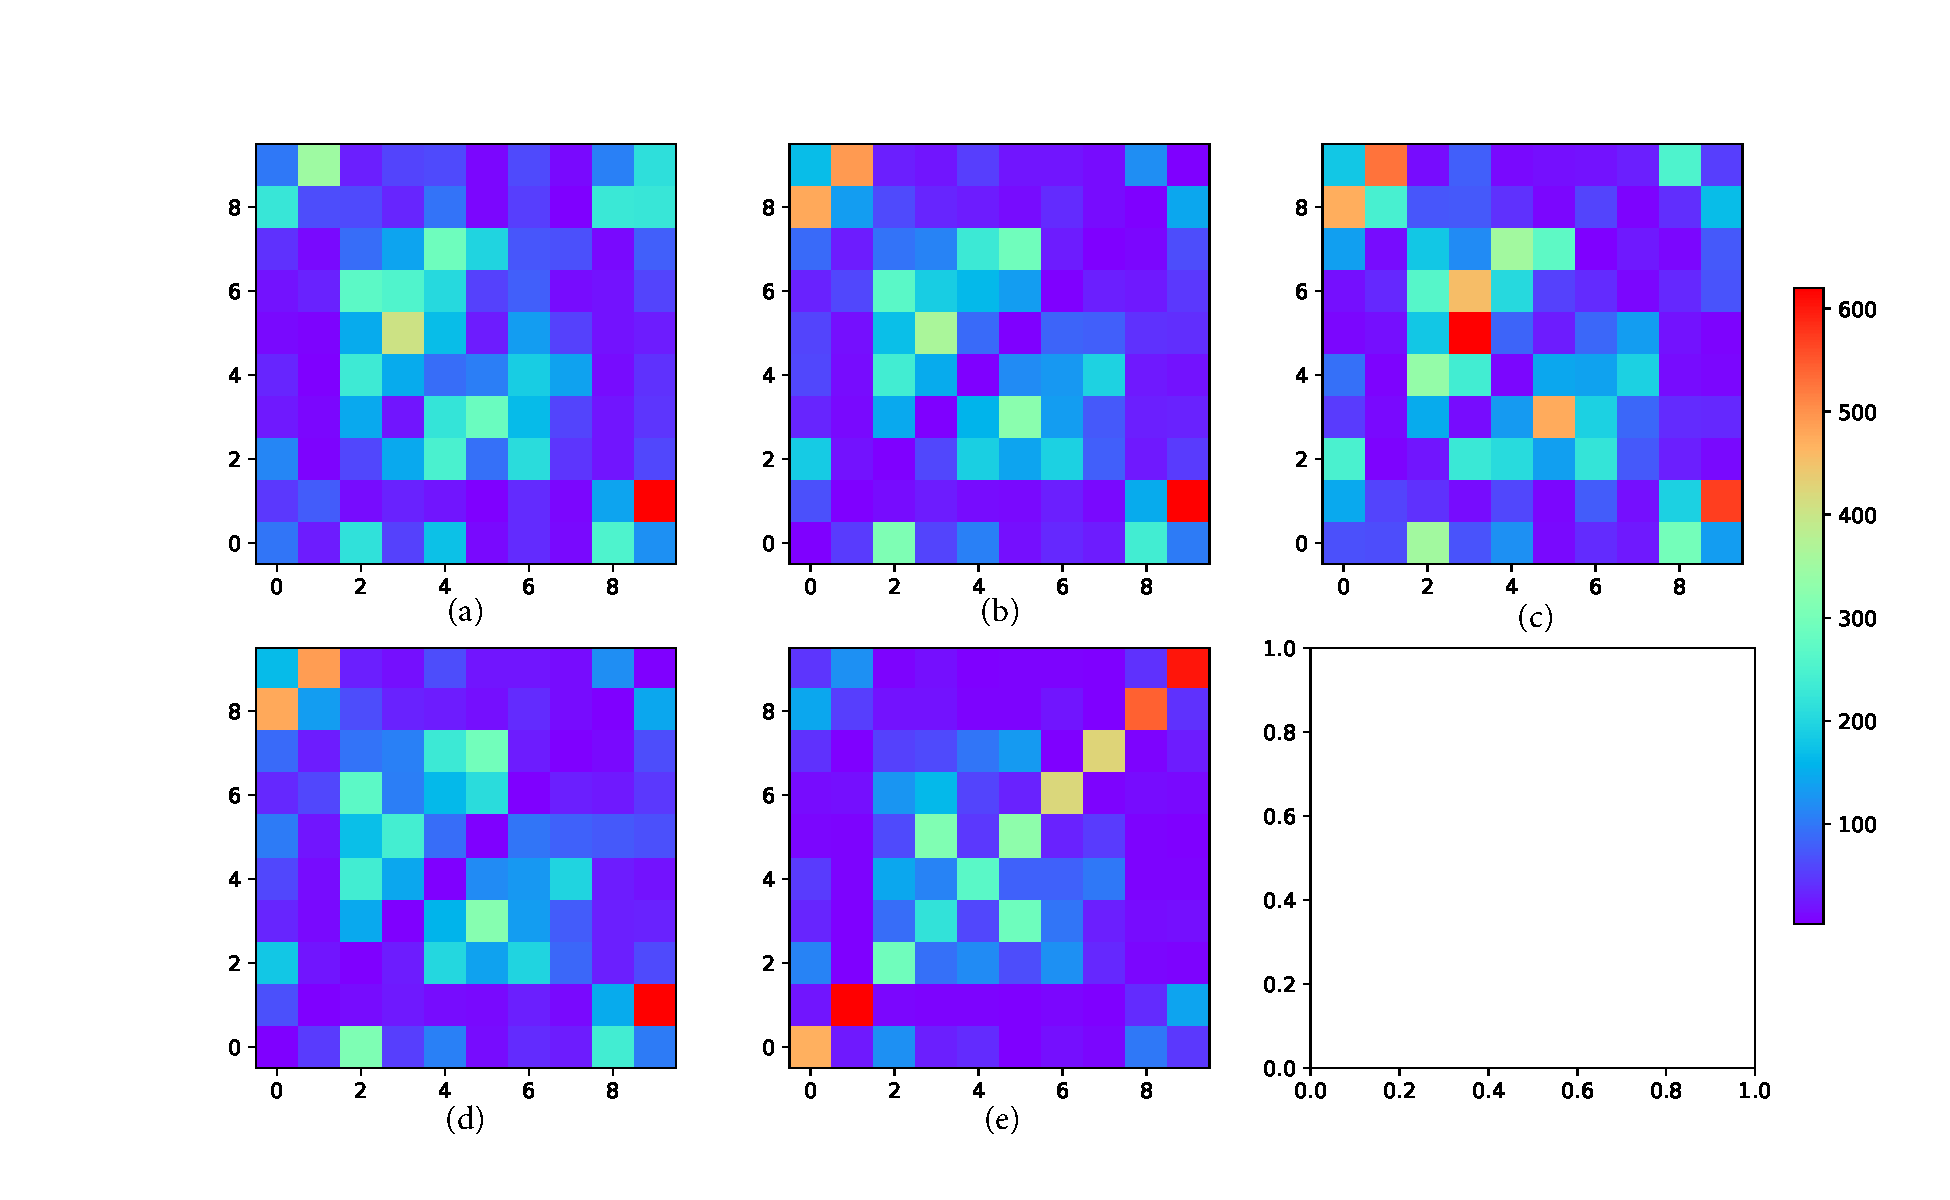
\includegraphics[width=1\linewidth]{figure/20210917/hotmap_attack_matrix.pdf}
    \caption{x-axis: origin category, y-axis: misleading category. Figures from a to e are
    generated by fgsm~\cite{fgsm}, bim~\cite{ifgsm}, 
    deepfool~\cite{deepfool}, pgd~\cite{pgd}, cw~\cite{cw} respectively.}
  \end{figure}
\end{frame}

\subsection{20210924}
\begin{frame}
  I evaluated a pretrained fastdepth model~\cite{fastdepth} using NYU
  depthv2~\cite{nyudepthv2} images shot by a phone camera.  

  \begin{figure}
    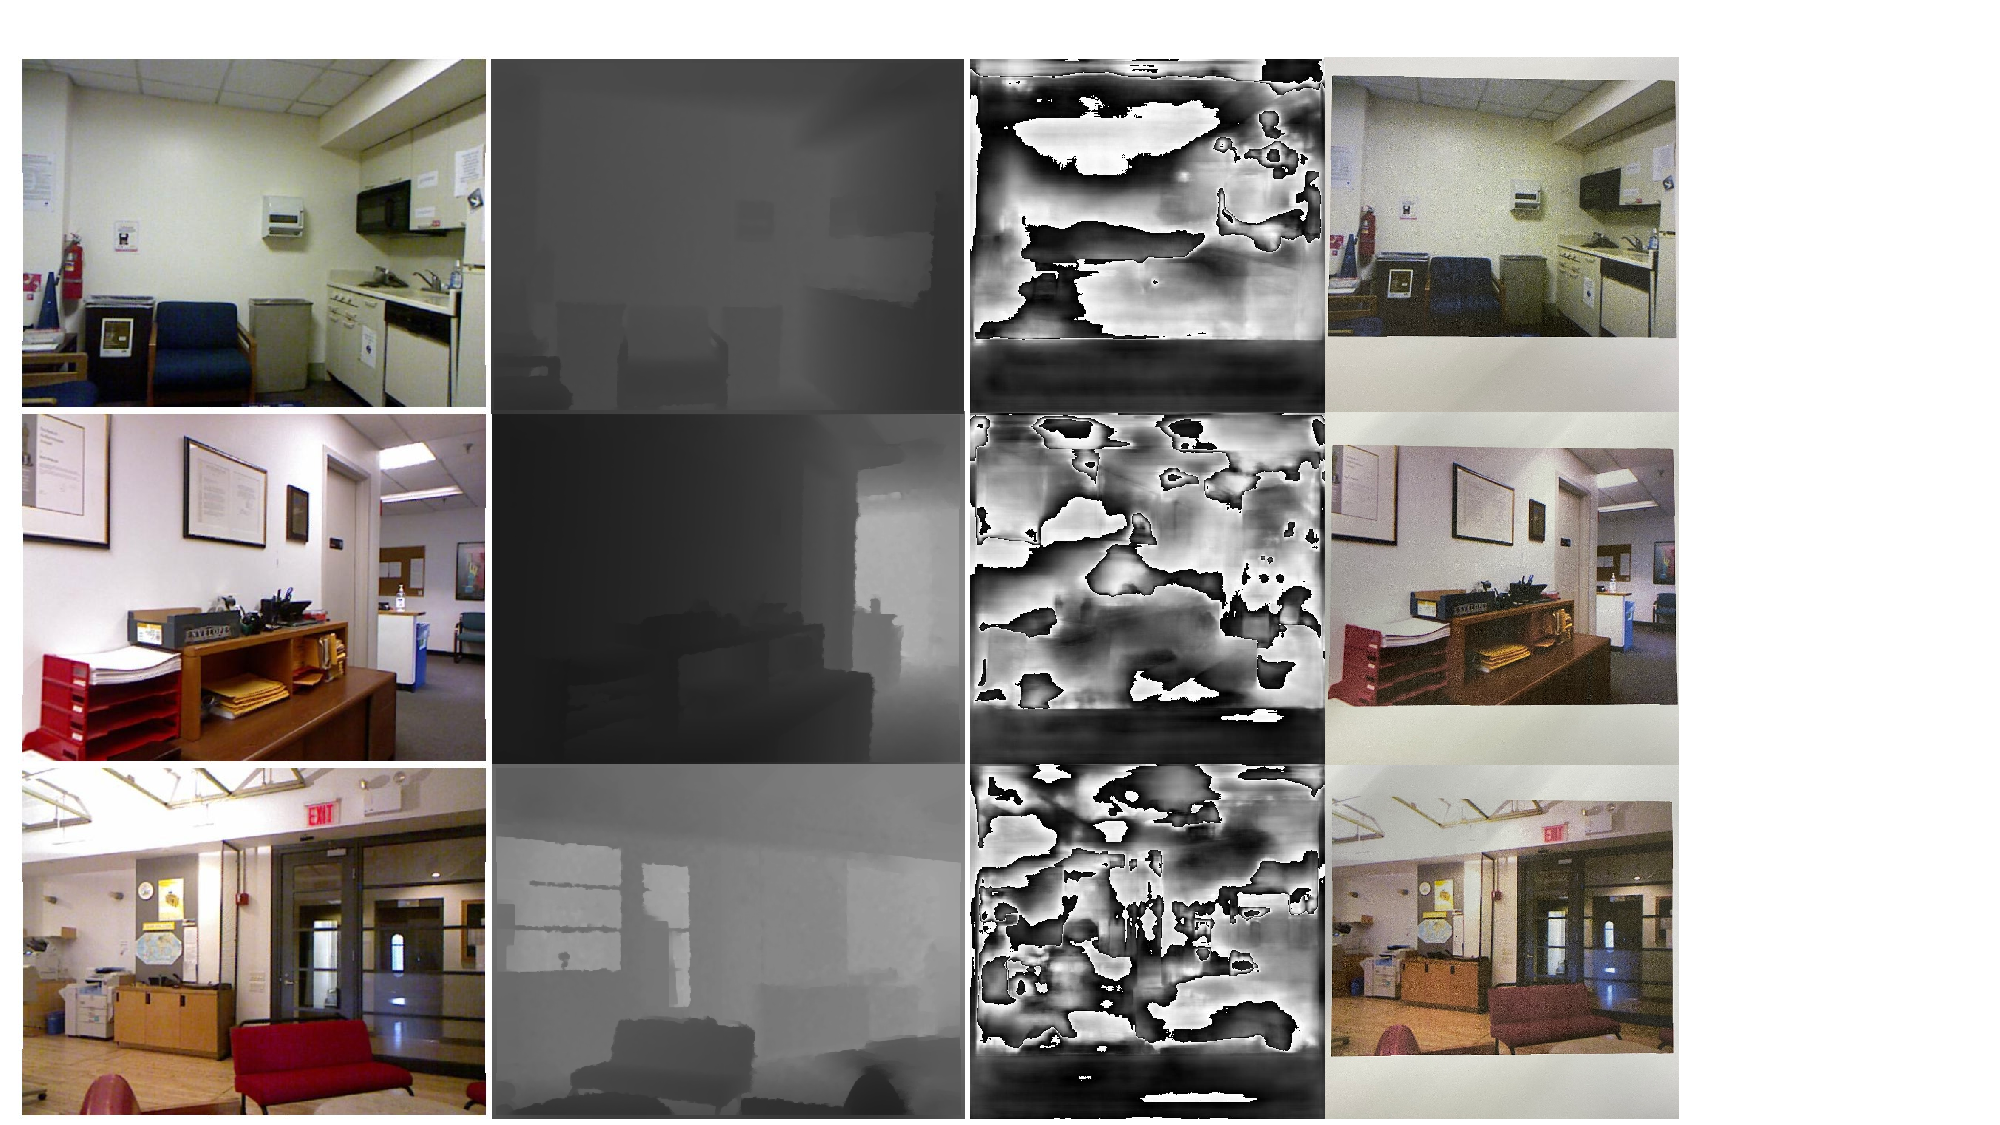
\includegraphics[width=1\linewidth]{figure/20210924/depth_real_1.pdf}
  \end{figure}
  \end{frame}

\begin{frame}
  \begin{figure}
    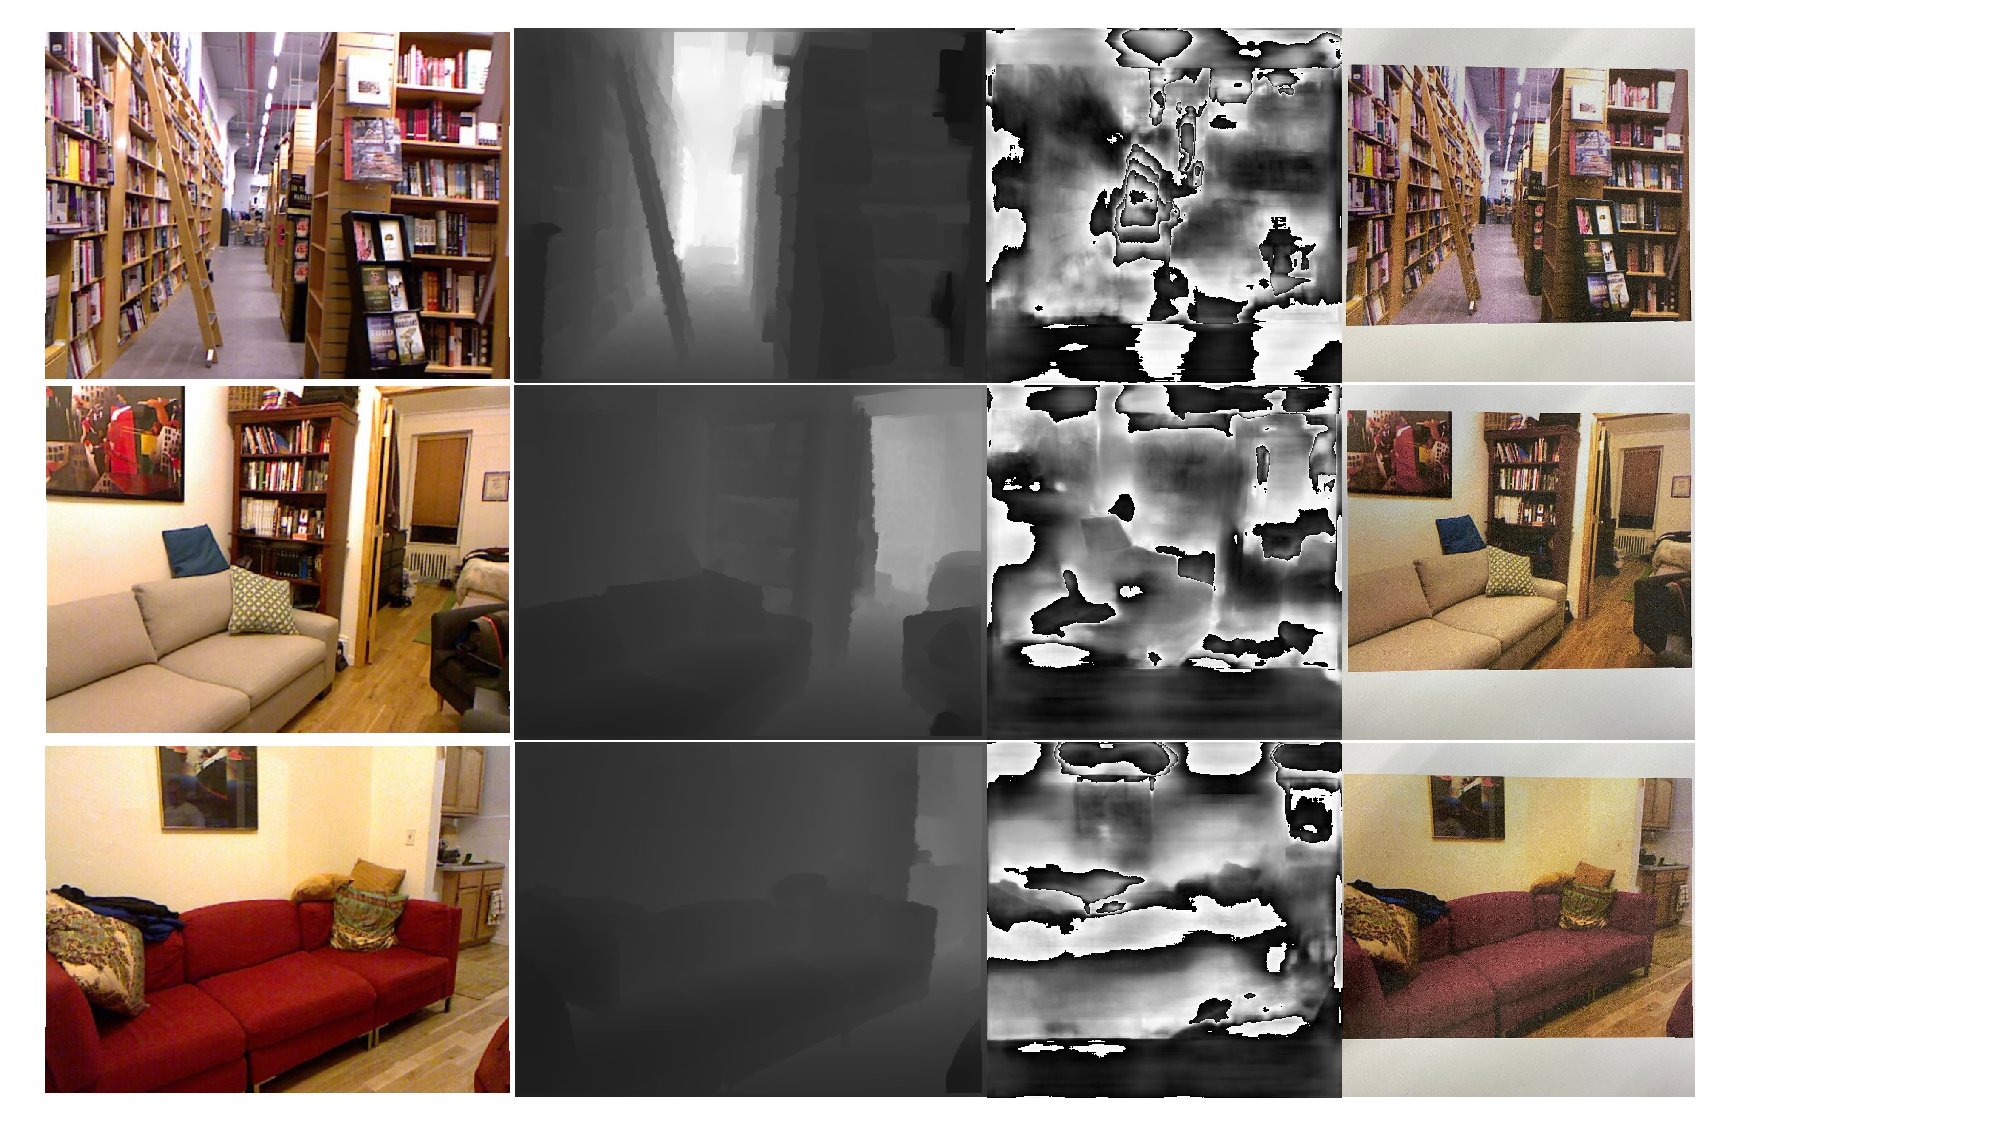
\includegraphics[width=1\linewidth]{figure/20210924/depth_real_2.pdf}
  \end{figure}
\end{frame}

\subsection{20211015}
\begin{frame}
  I evaluated a pretrained fastdepth model~\cite{fastdepth} using NYU
  depthv2~\cite{nyudepthv2} images shot by a phone camera.  
  \begin{figure}
    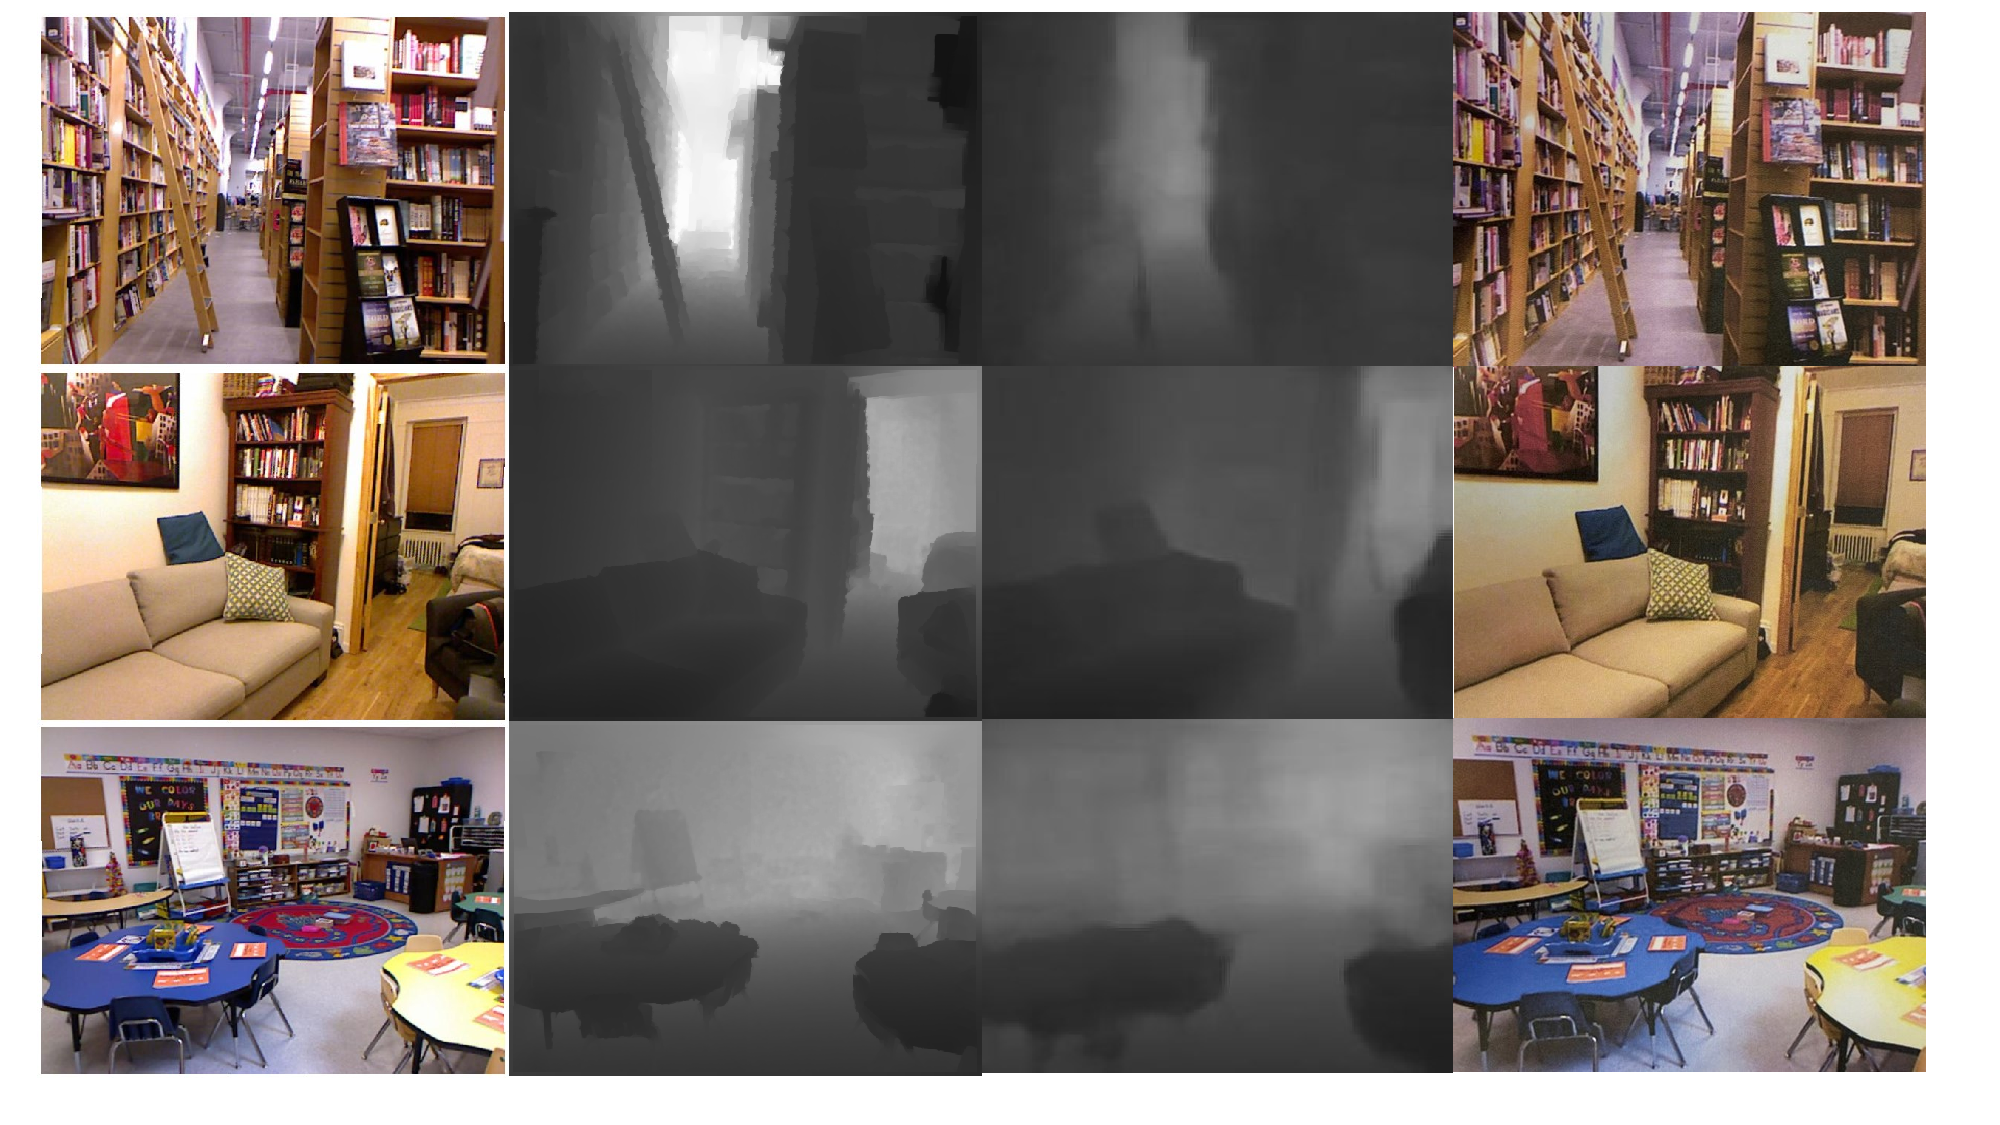
\includegraphics[width=1\linewidth]{figure/20211015/result1.pdf}
    \caption{results of print attack on fastdepth~\cite{fastdepth}
    using NYUdepthv2~\cite{nyudepthv2}.}
  \end{figure}
\end{frame}

\begin{frame}
  \begin{figure}
    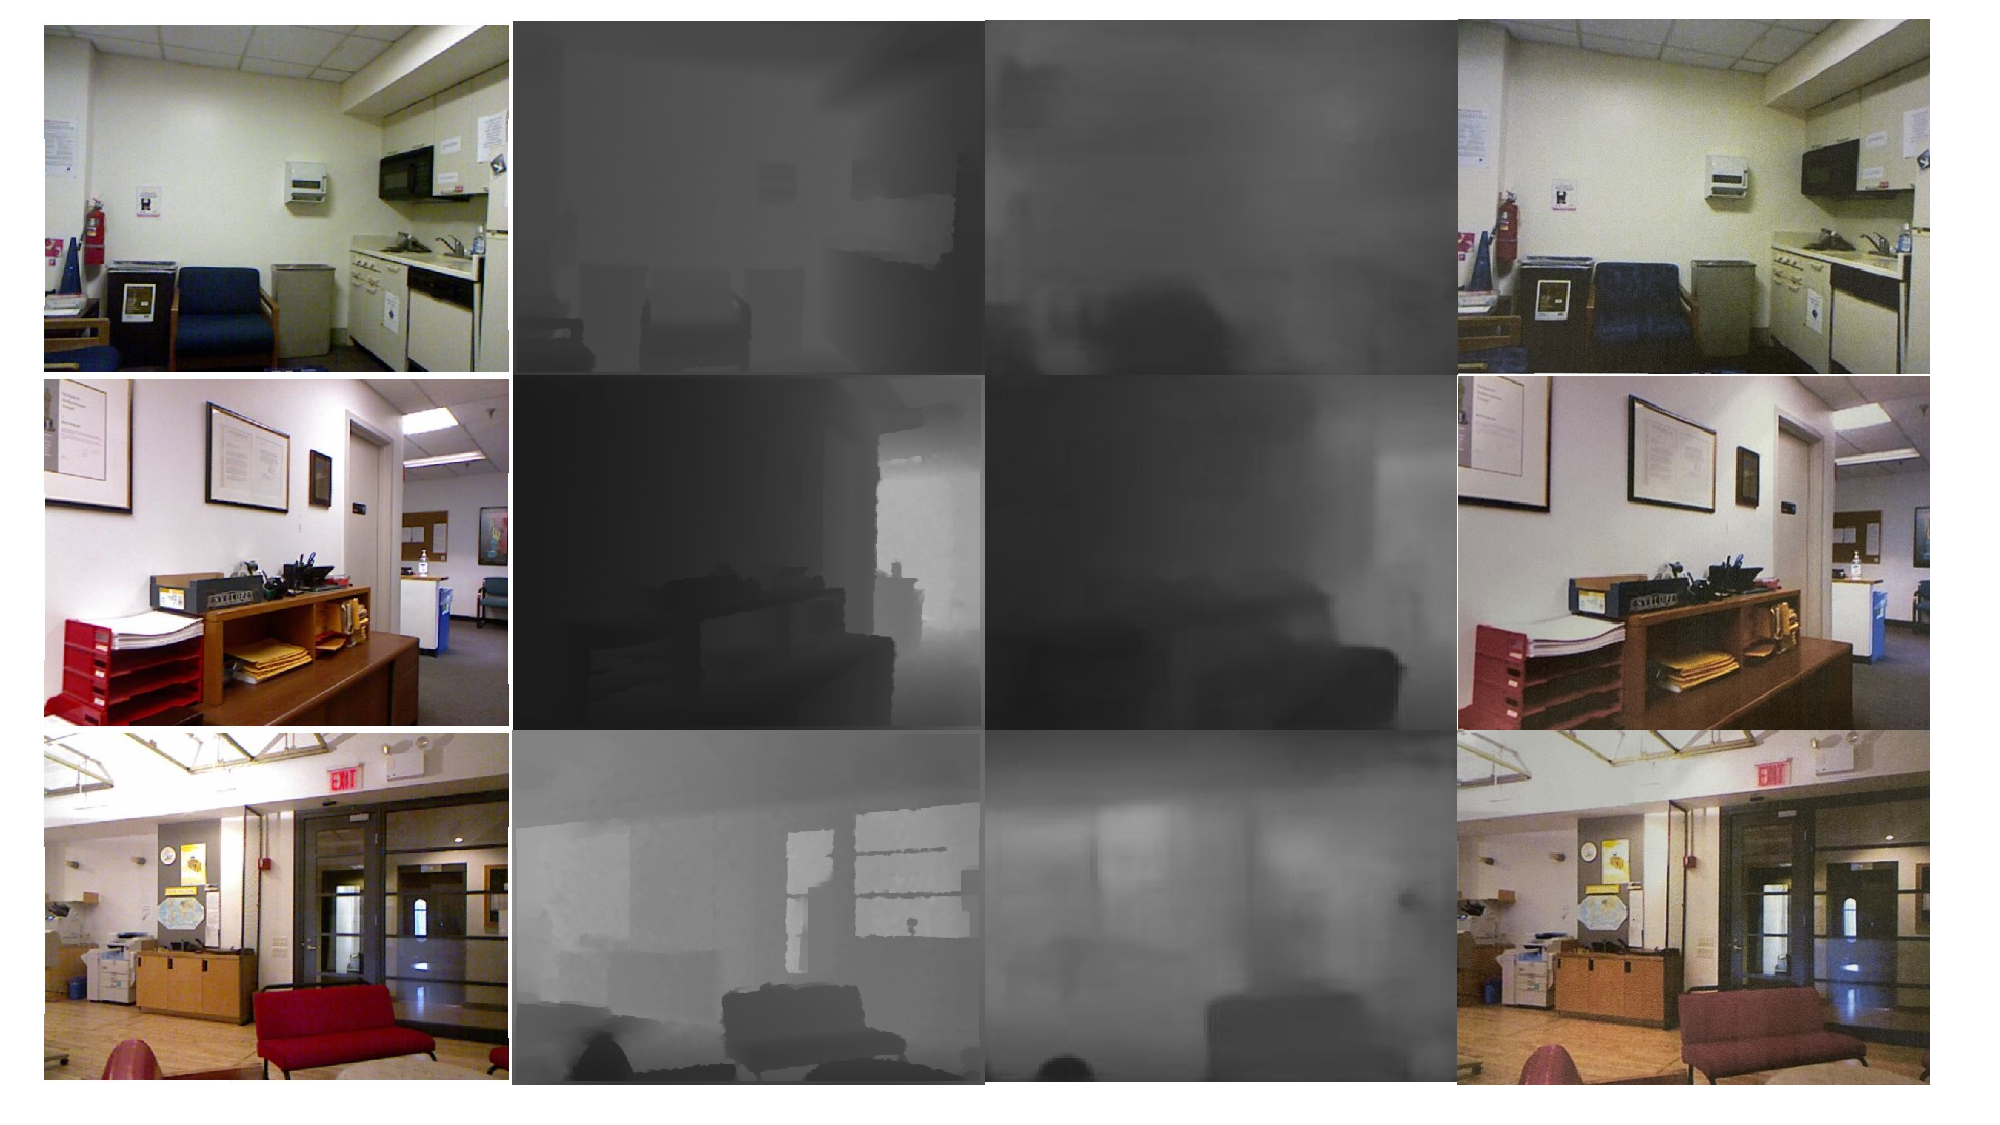
\includegraphics[width=1\linewidth]{figure/20211015/result2.pdf}
    \caption{results of print attack on fastdepth~\cite{fastdepth}
    using NYUdepthv2~\cite{nyudepthv2}.}
  \end{figure}
\end{frame}

\subsection{20211029}
\begin{frame}
  Experiment Preparation:
  \begin{figure}
    \subfigure[quick draw]{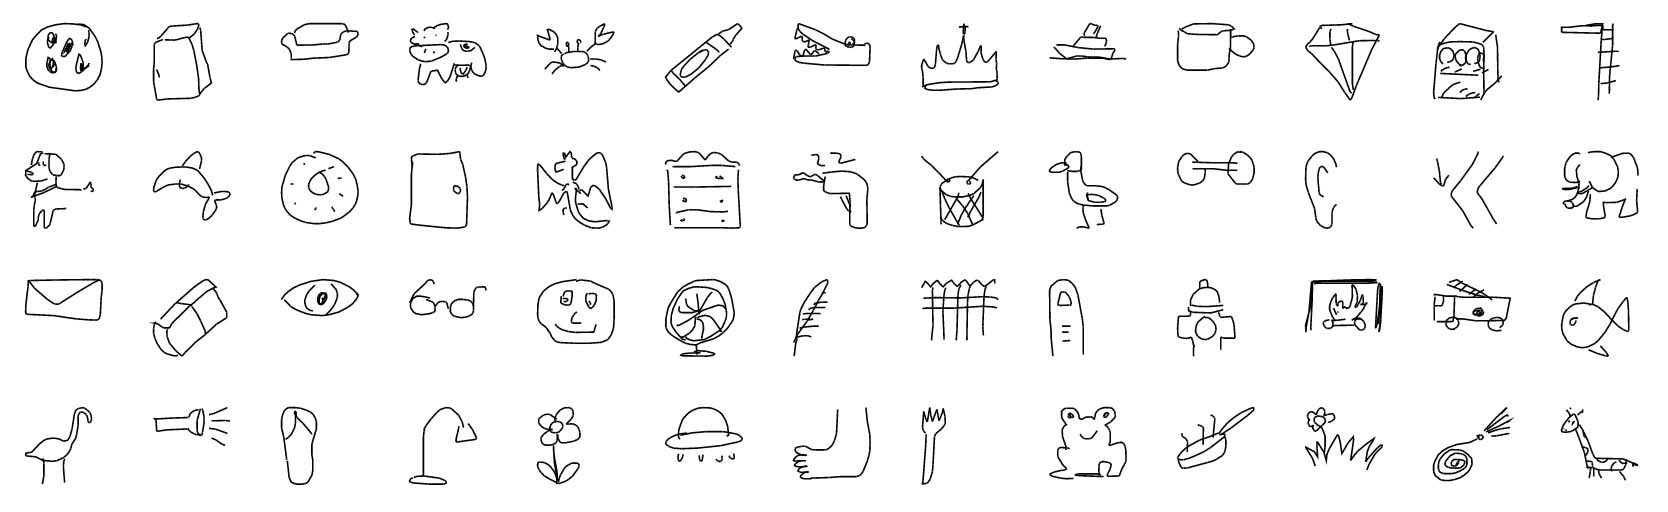
\includegraphics[width = 0.8\linewidth]{figure/20211029/preview.jpg}
}
    \subfigure[40 labels of NYUdepthv2~\cite{nyudepthv2}]{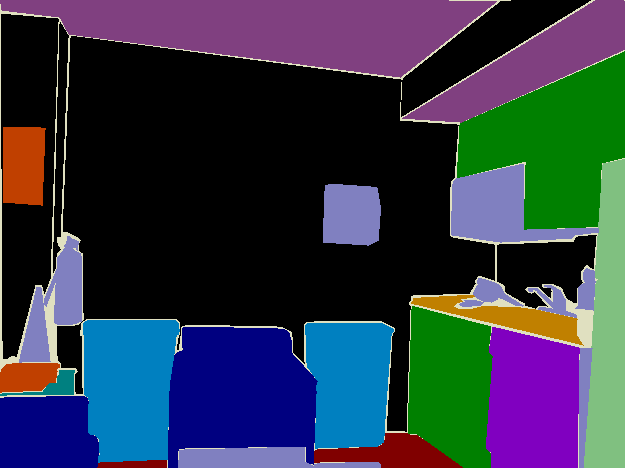
\includegraphics[width=0.5\linewidth]{figure/20211029/000001.png}
}
      \end{figure}
\end{frame}
\begin{frame}
 Experiment design:
 \begin{figure}
   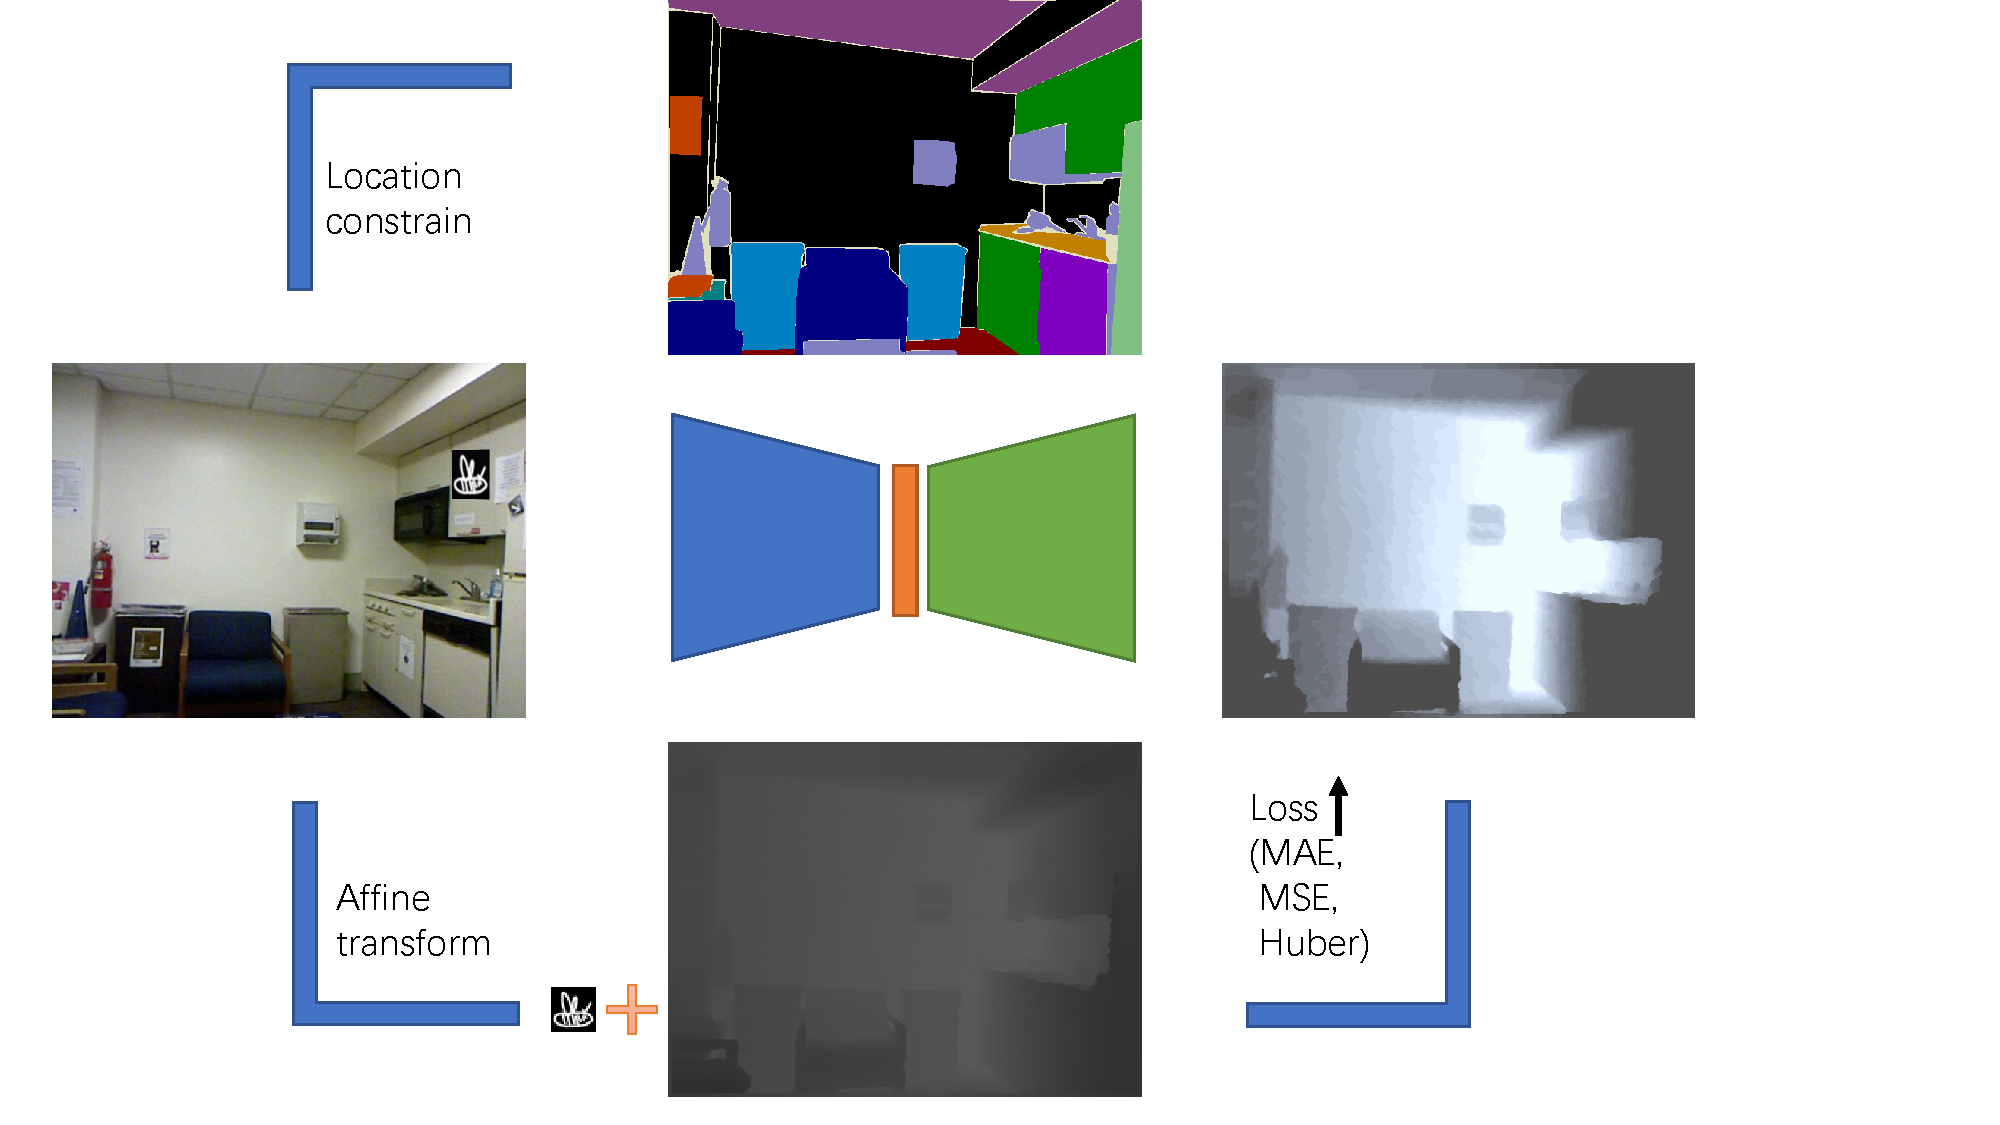
\includegraphics[width=1\linewidth]{figure/20211029/stream.pdf}
    \caption{Stream of our padding attack algorithm.}
 \end{figure}
\end{frame}

\subsection{20211112}
\begin{frame}
  Results of patch attack constrained by semantic information.
  \begin{table}
    \centering  % 显示位置为中间
    \caption{Accuracy of different attack method and original method}  % 表格标题
    \label{table1}  % 用于索引表格的标签
    %字母的个数对应列数,|代表分割线
    % l代表左对齐,c代表居中,r代表右对齐
    \begin{tabular}{c|c|c|c|c}  
      \hline  % 表格的横线
      &RMSE&MAE&absrel&delta1 \\  % 表格中的内容,用&分开,\\表示下一行
      \hline
      %& & & \\[-6pt]  %可以避免文字偏上 
      fastdepth~\cite{fastdepth}&0.600&0.427&0.162&0.771 \\
      random patch attack&0.674&0.564&0.177&0.743 \\
      ours patch attack&0.608&0.431&0.165&0.769 \\
      \hline
    \end{tabular}
  \end{table}
\end{frame}

\subsection{20211217}
\begin{frame}
  Results of patch attack constrained by semantic information.
  \begin{figure}
    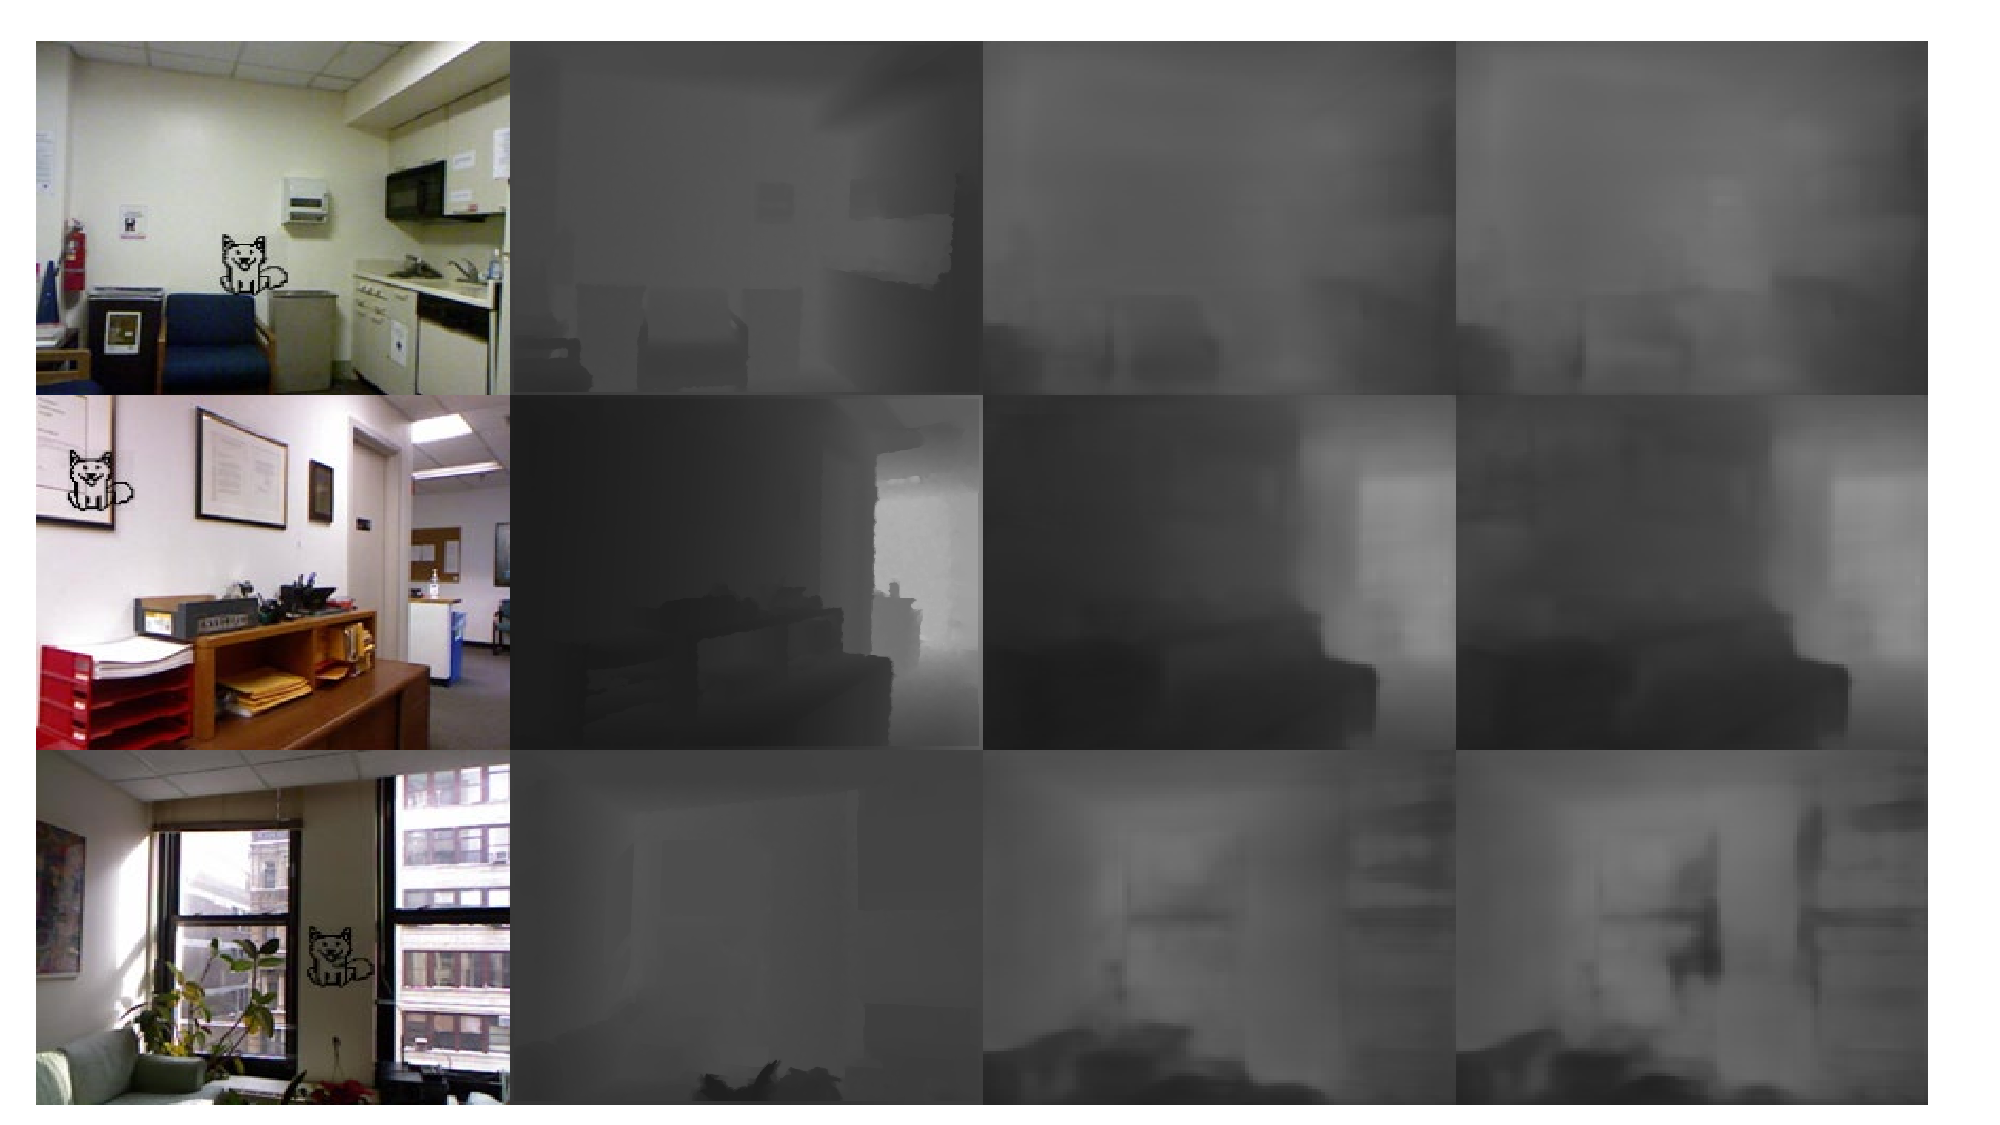
\includegraphics[width=1\linewidth]{figure/20211217/automatic_update_patch_result.pdf}
    \caption{results of automatic update patch attack on fastdepth~\cite{fastdepth}
    using NYUdepthv2~\cite{nyudepthv2}. From left to right are RGB images, ground truth depth,
    original NYUdepthv2 results and ours with patch attack respectively.}
  \end{figure}

\end{frame}

\begin{frame}
  Results of patch attack constrained by semantic information.
  \begin{figure}
    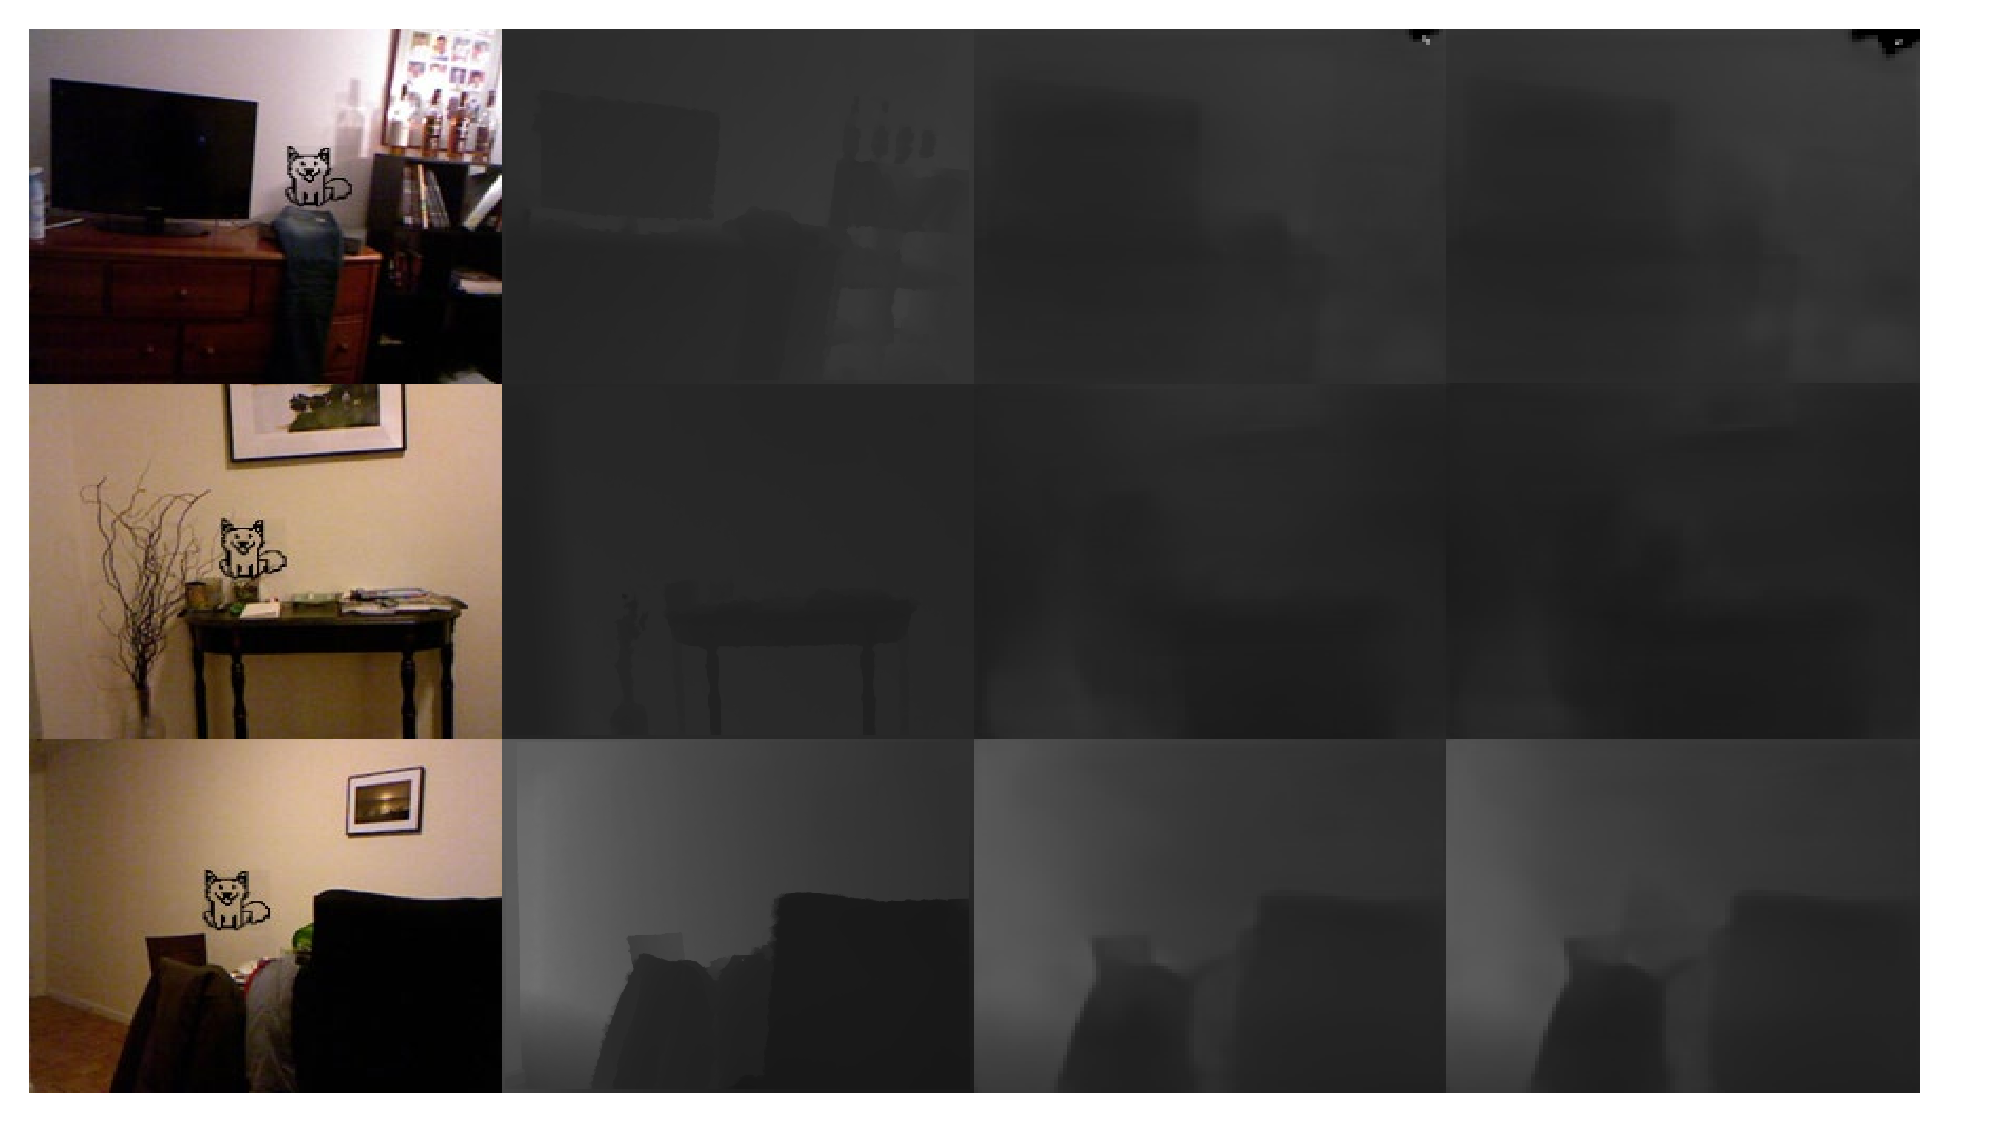
\includegraphics[width=1\linewidth]{figure/20211217/automatic_update_patch_attack2.pdf}
    \caption{results of automatic update patch attack on fastdepth~\cite{fastdepth}
    using NYUdepthv2~\cite{nyudepthv2}.}
  \end{figure}
\end{frame}

\begin{frame}
  Results of patch attack constrained by semantic information.
  \begin{table}
    \centering  % 显示位置为中间
    \caption{Accuracy of different attack method and original method}  % 表格标题
    \label{table2}  % 用于索引表格的标签
    %字母的个数对应列数,|代表分割线
    % l代表左对齐,c代表居中,r代表右对齐
    \begin{tabular}{c|c|c|c|c}  
      \hline  % 表格的横线
      &RMSE&MAE&absrel&delta1 \\  % 表格中的内容,用&分开,\\表示下一行
      \hline
      %& & & \\[-6pt]  %可以避免文字偏上 
      fastdepth~\cite{fastdepth}&0.600&0.427&0.162&0.771 \\
      random patch attack&0.674&0.564&0.177&0.743 \\
      ours patch attack&0.711&0.505&0.194&0.708 \\
      \hline
    \end{tabular}
  \end{table}
\end{frame}

\subsection{20220223}
\begin{frame}
  Results of attack on MDE using perspective transformed pathch.
  \begin{figure}
    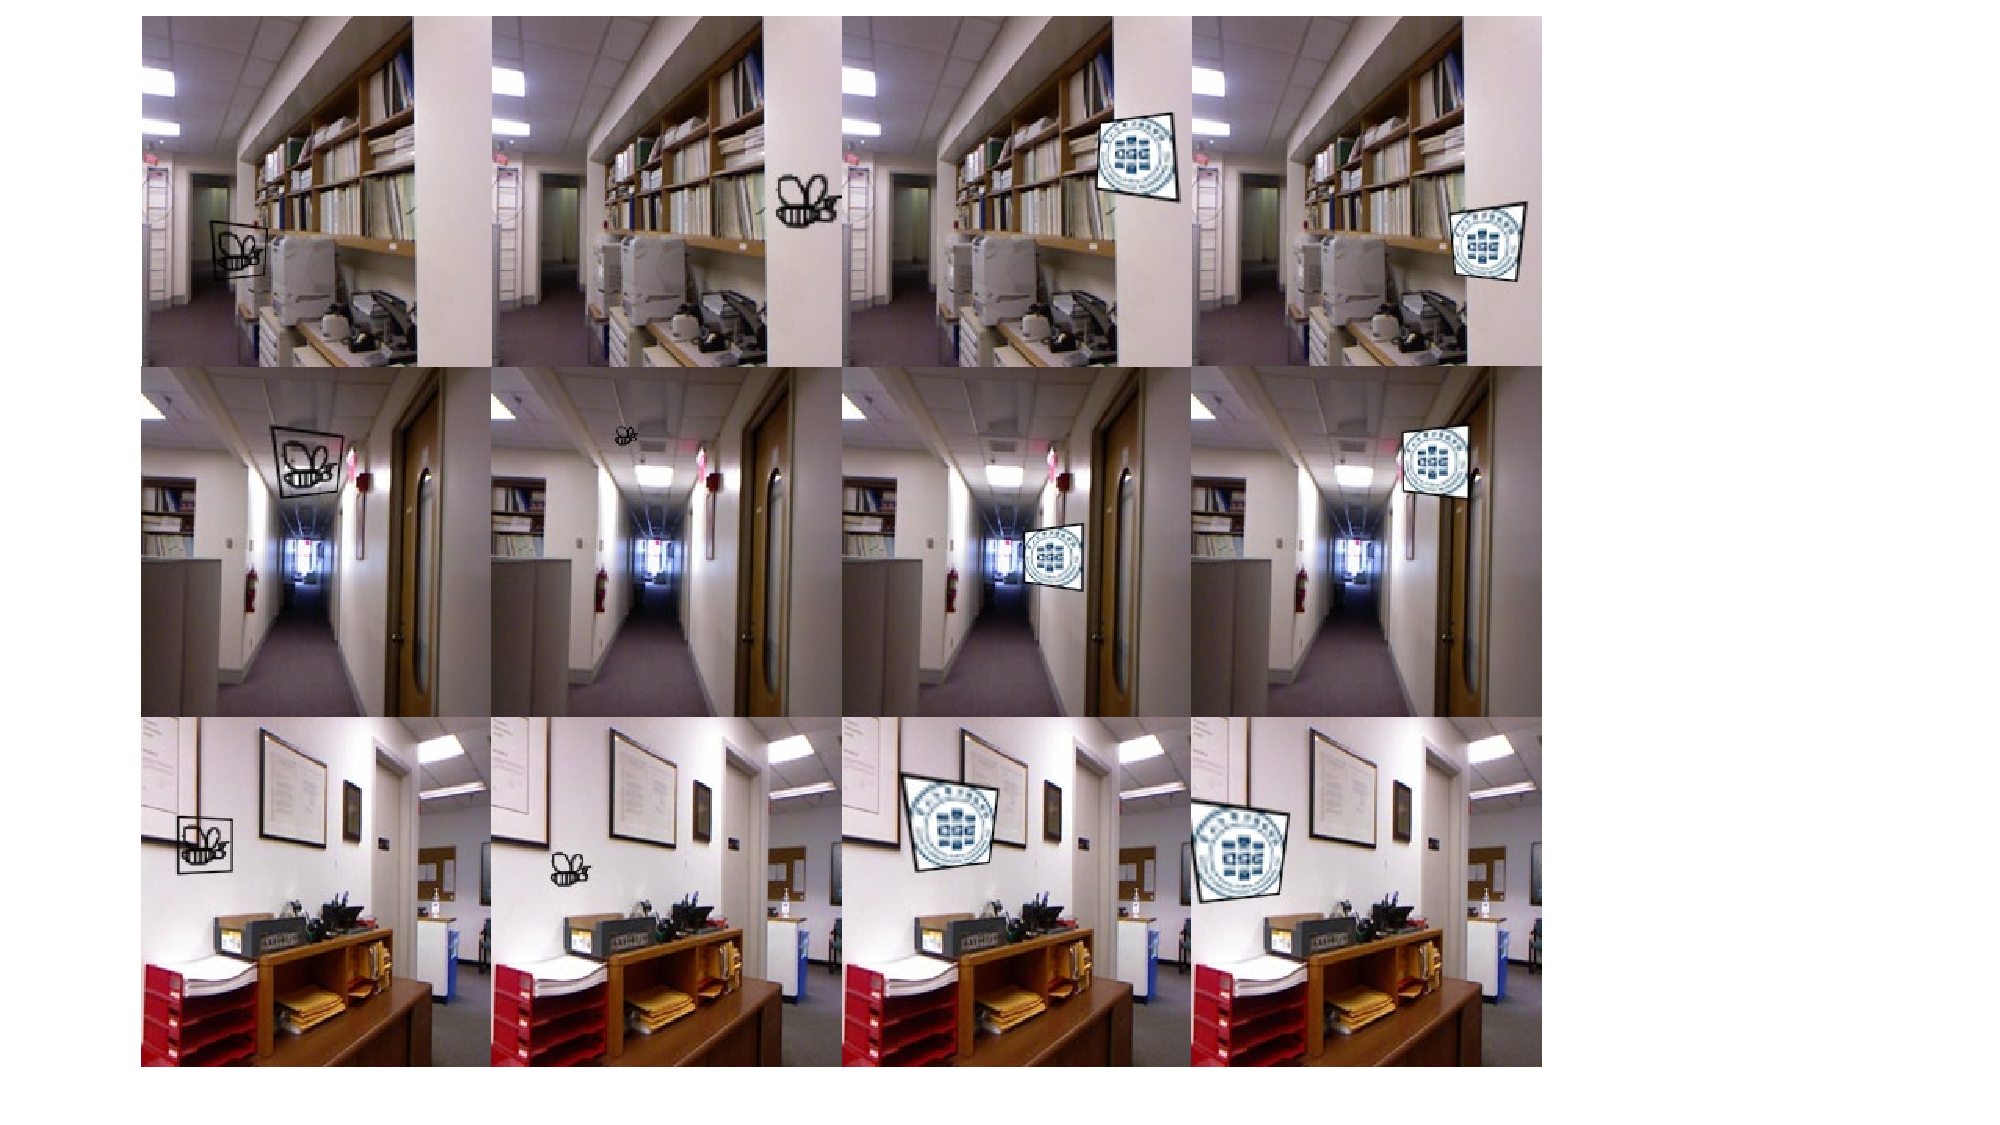
\includegraphics[width=1\linewidth]{figure/20220223/AttackMDE_01.pdf}
  \end{figure}
\end{frame}
\begin{frame}
  Results of attack on MDE using perspective transformed pathch.
  \begin{figure}
    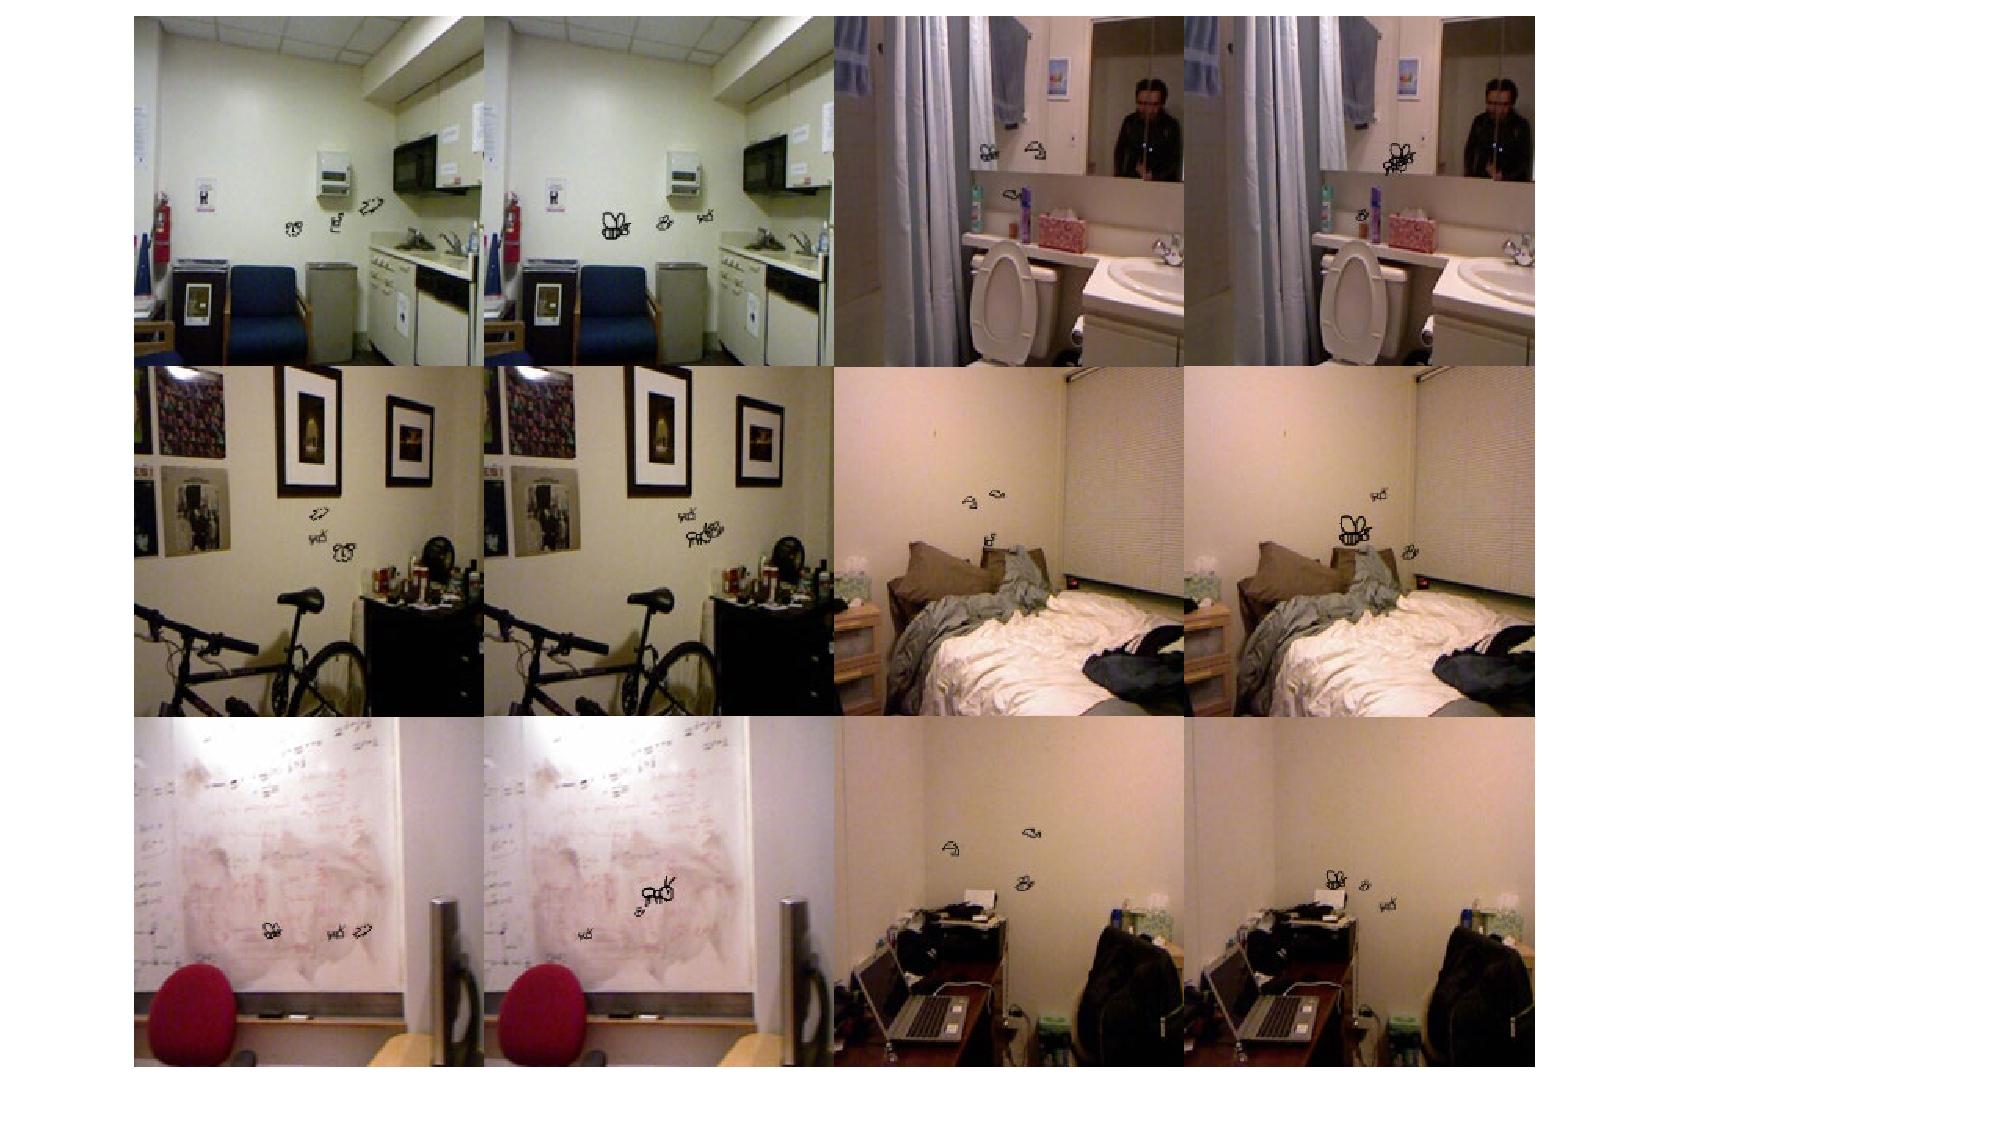
\includegraphics[width=1\linewidth]{figure/20220223/AttackMDE_02.pdf}
  \end{figure}
\end{frame}
  %\begin{figure}
  %  \subfigure[]{
  %    \begin{minipage}{0.2\linewidth}
  %       
\includegraphics[width=1\linewidth]{figure/20210924/00000_colors.png}
  %       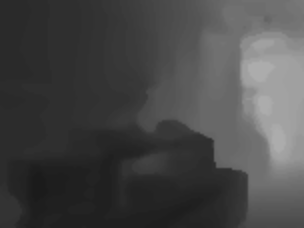
\includegraphics[width=1\linewidth]{figure/20210924/00008_colors.png}
  %       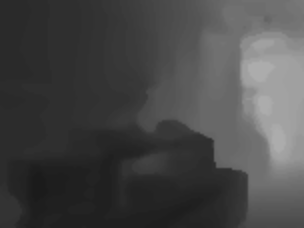
\includegraphics[width=1\linewidth]{figure/20210924/00008_colors.png}
  %    \end{minipage}}
  %  \subfigure[]{
  %    \begin{minipage}{0.2\linewidth}
  %       
\includegraphics[width=1\linewidth]{figure/20210924/00000_colors.png}
  %       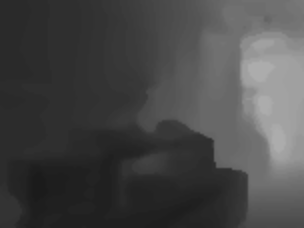
\includegraphics[width=1\linewidth]{figure/20210924/00008_colors.png}
  %       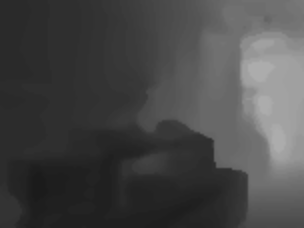
\includegraphics[width=1\linewidth]{figure/20210924/00008_colors.png}
  %    \end{minipage}
  %  }
  %\end{figure}

\section{References}

\begin{frame}[fragile]{Metropolis}

  The \themename theme is a Beamer theme with minimal visual noise
  inspired by the \href{https://github.com/hsrmbeamertheme/hsrmbeamertheme}{\textsc{hsrm} Beamer
  Theme} by Benjamin Weiss.

  Enable the theme by loading

  \begin{verbatim}    \documentclass{beamer}
    \usetheme{metropolis}\end{verbatim}

  Note, that you have to have Mozilla's \emph{Fira Sans} font and XeTeX
  installed to enjoy this wonderful typography.
\end{frame}

\begin{frame}[allowframebreaks]{References}

  \bibliography{demo}
  

\end{frame}

\end{document}
